\chapter{Results}\label{section:results}
\begin{figure*}[b!]
	\centering
	\setlength\tabcolsep{2pt}
	\begin{tabular}[width=0.8\textwidth]{c|cc|cc|cc|}
		\rotatebox{90}{\hskip 6pt SHREC16'A}&
		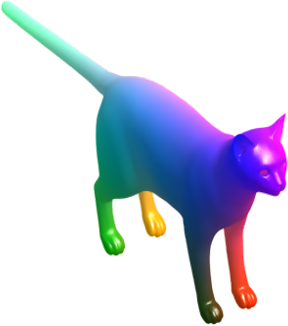
\includegraphics[scale=0.5]{figures/cat_base.png} &
		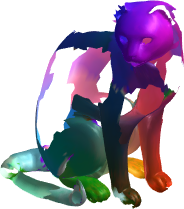
\includegraphics[scale=0.5]{figures/holes_cat_shape_16.png}  & 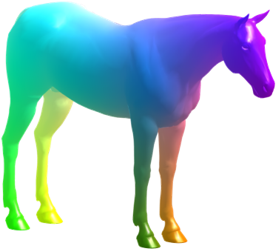
\includegraphics[scale=0.5]{figures/horse_base.png} & 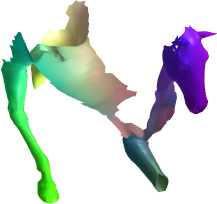
\includegraphics[scale=0.5]{figures/holes_horse_shape_5.png} &
		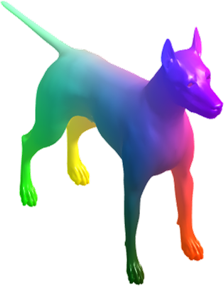
\includegraphics[scale=0.5]{figures/dog_base.png}&
		\multirow{1}{*}[1.2cm]{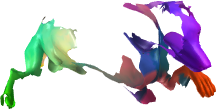
\includegraphics[scale=0.5]{figures/holes_dog_shape_9.png}}
		 %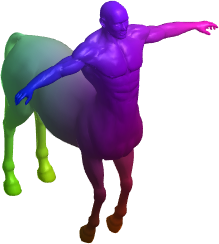
\includegraphics[scale=0.5]{figures/centaur_base.png}&
		%\multirow{1}{*}[1.5cm]{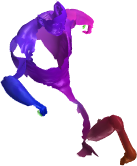
\includegraphics[scale=0.5]{figures/holes_centaur_shape_4.png}}
		\\ \hline
		\rotatebox{90}{\hskip 0.5cm SHREC16'B}&
		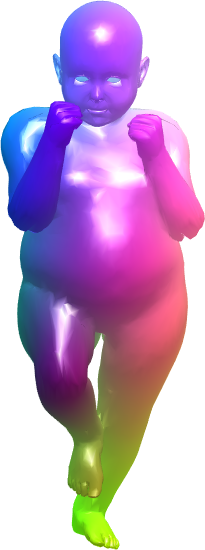
\includegraphics[scale=0.35]{figures/kid25-base.png} &
		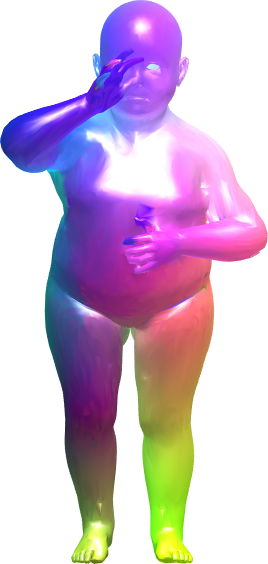
\includegraphics[scale=0.34]{figures/kid18match25.png} &
		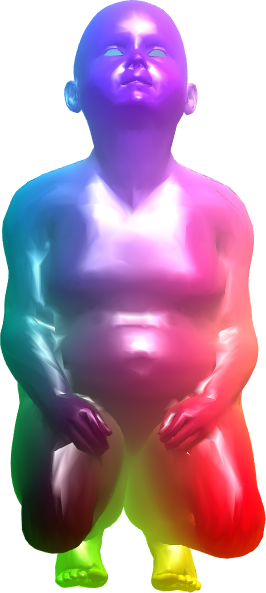
\includegraphics[scale=0.3]{figures/kid19_base.png}&
		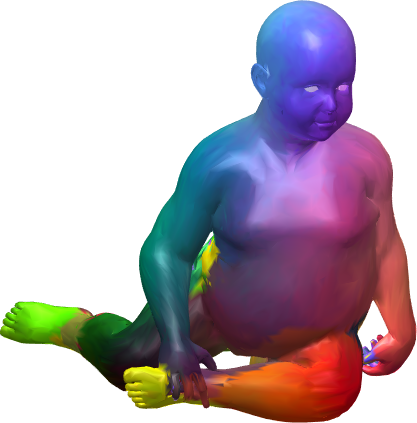
\includegraphics[scale=0.34]{figures/kid22_kid19.png}& 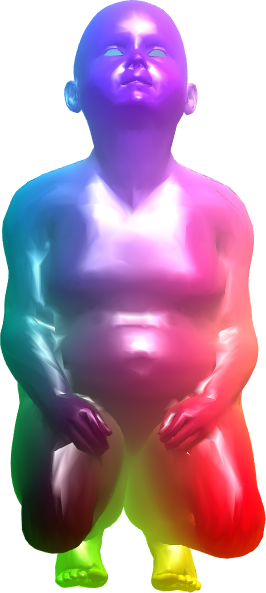
\includegraphics[scale=0.30]{figures/kid19_base.png} &
		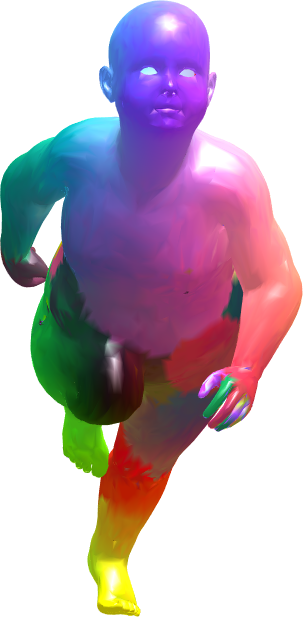
\includegraphics[scale=0.30]{figures/kid23_kid19.png} %&
		%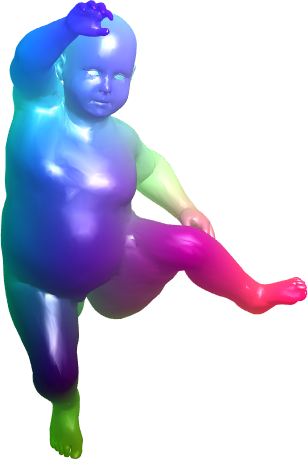
\includegraphics[scale=0.4]{figures/kid16.png} &
		%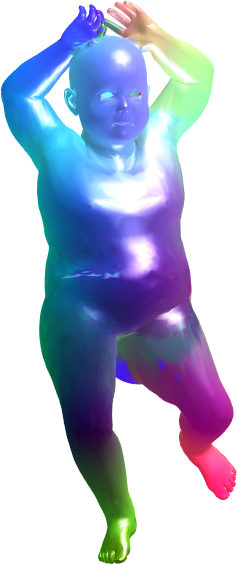
\includegraphics[scale=0.35]{figures/kid17_kid16.png}  
		\\ \hline
		\rotatebox{90}{\hskip 1.5cm FAUST}&
		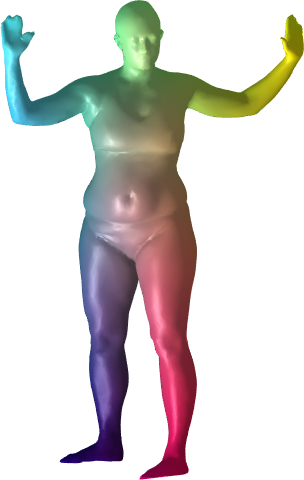
\includegraphics[scale=0.45]{figures/test_scan_035_base.png} &
		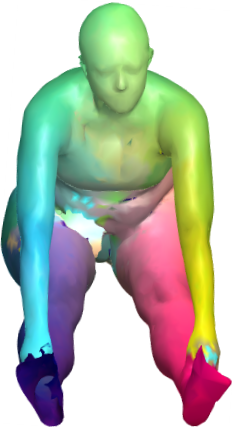
\includegraphics[scale=0.33]{figures/test_scan_035_test_scan_032.png}  & 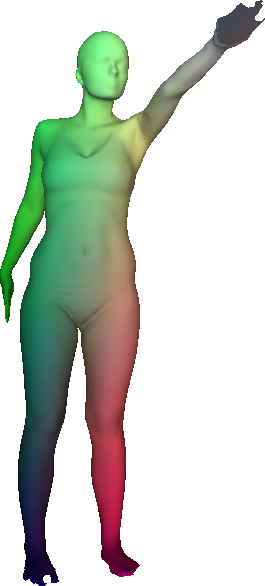
\includegraphics[scale=0.25]{figures/base01.png} &
		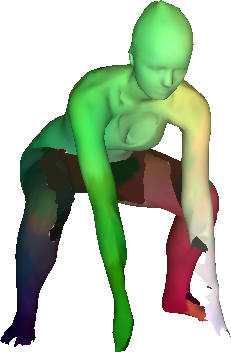
\includegraphics[scale=0.25]{figures/target00.png} &
		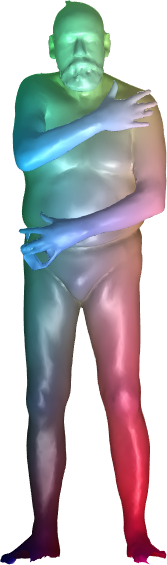
\includegraphics[scale=0.38]{figures/test_scan_051_bas.png}&
		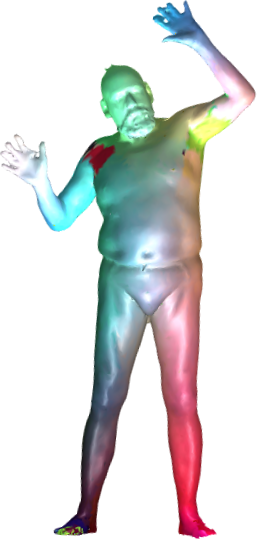
\includegraphics[scale=0.43]{figures/test_scan_051_test_scan_050.png}% &
		%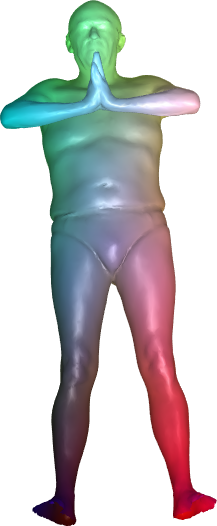
\includegraphics[scale=0.4]{figures/test_scan_066_base.png}&
		%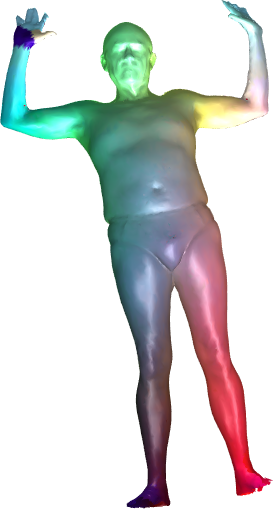
\includegraphics[scale=0.4]{figures/test_scan_066_test_scan_076.png} 
		\\ \hline
		& $\mathcal{M}$ & $\mathcal{N}$ & $\mathcal{M}$ & $\mathcal{N}$ & $\mathcal{M}$ & $\mathcal{N}$ %& $\mathcal{M}$ & $\mathcal{N}$
	\end{tabular}
	\caption{{\textbf {Results of our algorithm on examples from various datasets.}} 
			The corresponding points are colored in the same color.
			Note the accuracy of our algorithm in cases of symmetry (all), partiality (top), topological noise (middle) and large deformations (bottom).	
	}
	\label{fig:Shrec16Qualitative2}
\end{figure*}

We have evaluated our method both qualitatively and quantitatively on the two datasets of SHREC'16:
(1)~the benchmark of {\em SHREC'16A---partial matching of deformable shapes}~\cite{cosmo2016shrec};
(2)~the even more challenging benchmark of {\em SHREC'16B---matching of deformable shapes with topological noise}~\cite{lahner2016shrec}.
In both cases, our method either outperforms the results of state-of-the-art methods or is competitive.
In addition, we provide qualitative evaluation on challenging objects from {\em FAUST}~\cite{bogo2014faust};
see Figure~\ref{fig:Shrec16Qualitative2}.

{\em SHREC'16A} contains $400$ partial shapes, each is a near-isometrically deformed version of one of eight base models, given in a neutral pose.
The dataset is further divided into two subsets, according to the type of partiality:
(1) \textit{cuts}, which is composed of shapes produced by dividing shapes by a plane, and (2) \textit{holes}, obtained by eroding many areas around random vertices.
{\em SHREC'16B} contains $10$ shapes, which are derived from the same base human shape and underwent deformations and topological changes stemming from self-intersections.
{\em FAUST} contains $60$ pairs of high-resolution real-world scans of $10$ different human subjects. 
The acquisition process introduces topological artifacts and missing parts due to occlusions. 

Correspondence algorithms can be categorized into two classes, according to the density of the resulting correspondences: sparse and dense.
Dense-correspondences algorithms match every vertex on one shape to a vertex on the other shape.
Sparse-correspondence algorithms cover the surface by a sparse set of points and find correspondences only for them.

Our algorithm belongs to the latter class: it produces a sparse set of correspondences.
However, as a post-processing step, we can convert the set of sparse correspondences to a dense set using the method of~\cite{litany2017fully}.


\begin{figure*}[b!]
	\centering
	\setlength\tabcolsep{2pt}
	\begin{tabular}[width=0.8\textwidth]{c|ccc}
		input &  Rodola'17\cite{rodola2017partial} & ours-dense & ours-sparse
		\\ \hline
		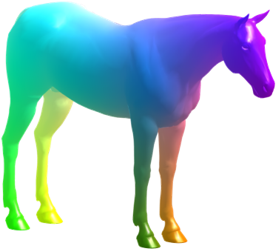
\includegraphics[scale=0.5]{figures/horse_base.png} & 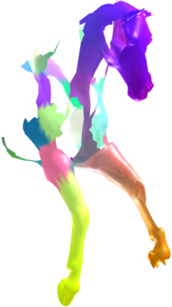
\includegraphics[scale=0.5]{figures/holes_horse_12_PFM.png}  & 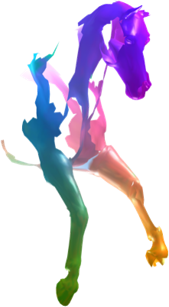
\includegraphics[scale=0.5]{figures/holes_horse_12.png} & 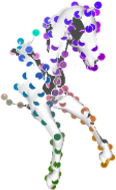
\includegraphics[scale=0.48]{figures/holes_horse_12_sparse.png}\\
		& 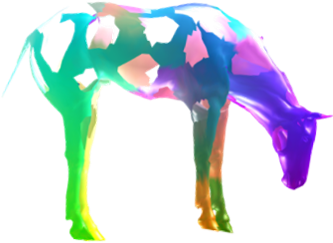
\includegraphics[scale=0.5]{figures/holes_horse_16_PFM.png}&
		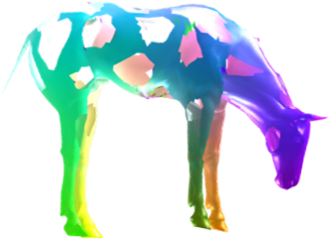
\includegraphics[scale=0.5]{figures/holes_horse_16.png} & 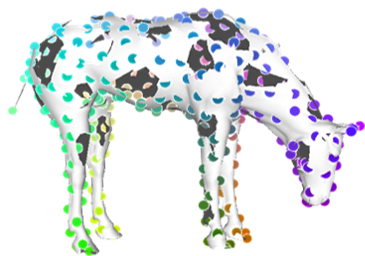
\includegraphics[scale=0.47]{figures/holes_horse_16_sparse.png} \\ \hline 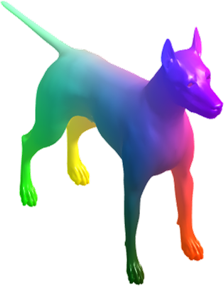
\includegraphics[scale=0.5]{figures/dog_base.png} &
		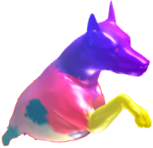
\includegraphics[scale=0.55]{figures/cuts_dog_8_PFM.png}  & 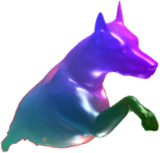
\includegraphics[scale=0.53]{figures/cuts_dog_8.png} & 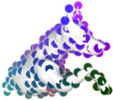
\includegraphics[scale=0.48]{figures/cuts_dog_8_sparse.png}\\ & 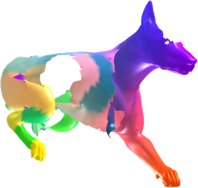
\includegraphics[scale=0.55]{figures/holes_dog_13_PFM.png} & 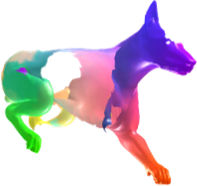
\includegraphics[scale=0.53]{figures/holes_dog_13.png} &
		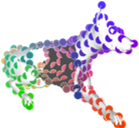
\includegraphics[scale=0.5]{figures/holes_dog_13_sparse.png}\\
	\end{tabular}
	\caption{{\textbf {Results on examples from SHREC'16A.}}
	The left column shows the input model in a neutral pose.
The other columns compare our results (both dense and sparse) to the SOTA results of~\cite{rodola2017partial}, for which the code is gratefully provided.
The models are partial, deformed and have many holes.
Our results outperform those of~\cite{rodola2017partial}, when run with the default parameters.
For instance, the front leg of the dog has the correct color in our result, whereas the result of~\cite{rodola2017partial} matched it to the rear leg (in yellow).
	}
	\label{fig:Shrec16Qualitative}
\end{figure*}


%%%%%%%%%%%%%%%%%%%%%% Qualitative results %%%%%%%%%%%%%%%%%%%
\paragraph{Qualitative results}
Figure~\ref{fig:Shrec16Qualitative2} illustrates our results on various shapes, which contain symmetries, large deformations, partiality and topological noise.
In this figure, the input model $\mathcal{M}$ is color-coded according to the coordinates of the vertices.
The matches on the target model $\mathcal{N}$  are colored according to the color of their corresponding vertices.
Therefore, it is easy to visually verify the accuracy of our results, by comparing the color "by eye".

Figure.~\ref{fig:Shrec16Qualitative} compares our dense-correspondence results  from {\em SHREC'16A} to those of~\cite{rodola2017partial} (which computes dense correspondence directly).
Our method produces better results especially in cases of symmetries (e.g., the legs).
This is due to distance preservation between points in Equation~\ref{eq:DDIS}.
This is particularly important when the model contains holes.
This figure also demonstrates our results of sparse correspondence, where the dots on the model suit in color the matching parts of $\mathcal{M}$ .

Figure~\ref{fig:Shrec16Qualitative-error} further demonstrates the quality of our results, by color-coding the errors.
The larger the error, the more reddish the color is.
It can be seen  that our results hardly have any yellow/red, whereas the results of~\cite{rodola2017partial} have yellow/red regions.

\begin{figure*}[h!]
	\centering
	\setlength\tabcolsep{0.5pt}
	\begin{tabular}[width=0.8\textwidth]{cc|ccc}
		Rodola'17\cite{rodola2017partial} & Ours
		&  Rodola'17\cite{rodola2017partial} & Ours& \\ \hline
		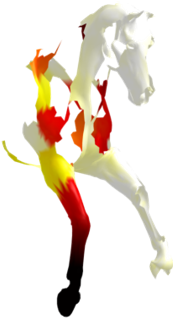
\includegraphics[scale=0.5]{figures/holes_horse_12_err_PFM.png} & 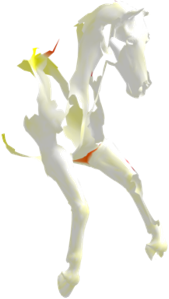
\includegraphics[scale=0.5]{figures/holes_horse_12_err.png} &  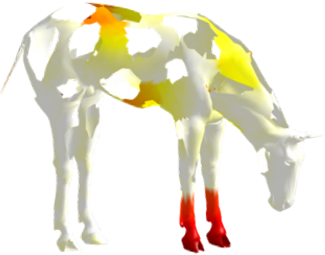
\includegraphics[scale=0.5]{figures/holes_horse_16_err_PFM.png}&
		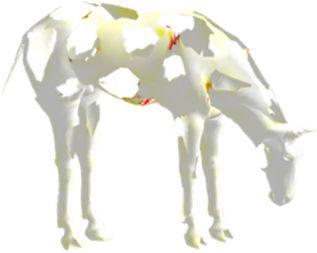
\includegraphics[scale=0.5]{figures/holes_horse_16_err.png}&\multirow{2}{0.5cm}[2.3cm]{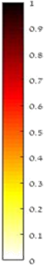
\includegraphics[scale=1]{figures/ErrorBar.png}} \\
		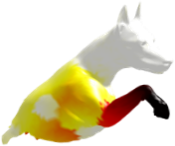
\includegraphics[scale=0.5]{figures/cuts_dog_8_err_PFM.png} &
		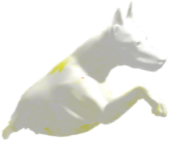
\includegraphics[scale=0.5]{figures/cuts_dog_8_err.png} &  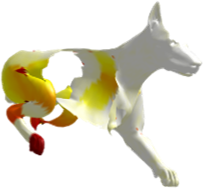
\includegraphics[scale=0.5]{figures/holes_dog_13_PFM_err.png}&   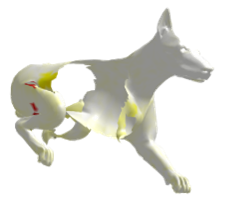
\includegraphics[scale=0.5]{figures/holes_dog_13_err.png}& \\
	\end{tabular}
	\caption{{\textbf {Errors on examples from SHREC'16A.}}
		The error is color-coded from white (no error) to red (large error).
		Our results evidently are less erroneous than those of ~\cite{rodola2017partial}.
	}
	\label{fig:Shrec16Qualitative-error}
	\end{figure*}
	
Similarly, Figure~\ref{fig:Shrec16TopImage} shows a couple of examples from {\em SHREC'16B}, where the models have topological noise, i.e. regions that should not intersect semantically, do intersect geometrically (e.g., the triangles of the face and the head intersect).
Generally, our method outperforms that of ~\cite{rodola2017partial}, having fewer and scarce failures.
Moreover, our failures are constrained to regions near the topological noise.
\begin{figure*}[h!]
	\centering
	\begin{tabular}{ccc}
		input  & Rodola'17\cite{rodola2017partial} & Ours \\
		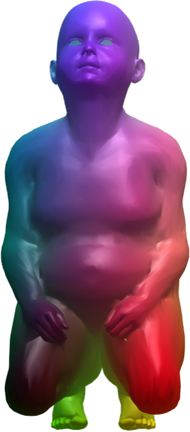
\includegraphics[scale=0.4]{figures/Top2Base.png} &
		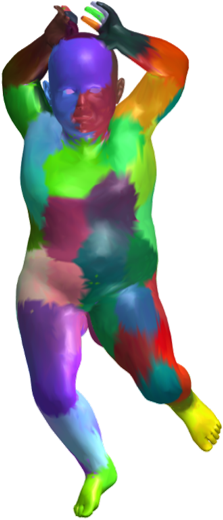
\includegraphics[scale=0.4]{figures/Top2PFM.png} &
		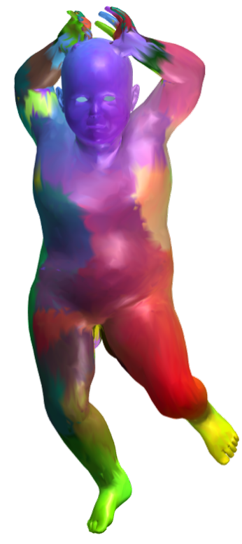
\includegraphics[scale=0.4]{figures/Top2DDIS.png} \\
		\includegraphics[scale=0.3]{figures/kid22_base.png} &
		\includegraphics[scale=0.2]{figures/kid23_kid22_PFM.png} &
		\includegraphics[scale=0.21]{figures/kid23_kid22.png}
	\end{tabular}
	\caption{{\textbf {Results on SHREC'16B.}}
		Top: the result of~\cite{rodola2017partial} contains more erroneous segments than ours (e.g., segments on the legs).
		Furthermore, our errors are more constrained to regions that indeed contain topological noise.
		Bottom: the legs are switched  in~\cite{rodola2017partial}, but not in our method.
		This is not only thanks to our similarity function that maintains distances, but also thanks to our multi-scale approach.
	}
	\label{fig:Shrec16TopImage}
\end{figure*}

Figure~\ref{fig:litani} compares our result to the reported failure case  of~\cite{litany2017deep}, which introduces a deep learning model.
It can be seen that our method is able to handle extreme partiality.




\begin{figure*}[h!]
	\centering
	\begin{tabular}{cc}
		input  & Litani'17B\cite{litany2017deep}\\
		\includegraphics[scale=0.7]{figures/litanibase.png} &
		\includegraphics[scale=0.7]{figures/Litanires.png} \\
		input & Ours \\
		\includegraphics[scale=0.7]{figures/dog_base.png} &
		\includegraphics[scale=0.7]{figures/LitaniOurs.png} \\
		
	\end{tabular}
	\caption{{\textbf {Comparison with~\cite{litany2017deep}}.}
		Our method manages to handle extreme partiality, compared to a result of a recent deep learning model.
	}
	\label{fig:litani}
\end{figure*}

%%%%%%%%%%%%%%%%   Quantitative results %%%%%%%%%%%%%%%%%%
\paragraph{Quantitative results}
Next, we provide a quantitative evaluation of our method on the above datasets w.r.t previously reported results.
The common error metric used in previous work is the {\em normalized geodesic distance (NGD)}~\cite{kim2011blended}.
NGD is defined as follows:
Let the corresponding point of $p \in \mathcal{N}$, as found by the algorithm, be $q \in \mathcal{M}$, and let the ground truth corresponding point of $p$ be $q^* \in \mathcal{M}$.
The error for $p$ is the normalized geodesic distance between  $q$ and $q^*$ on $\mathcal{M}$:
\begin{equation}
	\centering
	NGD(p)=\frac{GeoDist_{\mathcal{M}}(q,q^*)}{\sqrt{area(\mathcal{M})}}.
\end{equation}
\begin{figure*}[h!]
	\centering
	\setlength\tabcolsep{2pt}
	\begin{tabular}{ccc}
		& \small{SHREC'16A-Cuts} & \small{SHREC'16A-Holes} \\
		\rotatebox{90}{\hskip 5mm \, \% Correspondences} &
		\includegraphics[width=0.44\textwidth]{figures/Curves_Cuts.png} & \includegraphics[width=0.4\textwidth]{figures/Curves_Holes.png} \\
		& \small{NGD} & \small{NGD}\\[0.1in]
		%\multicolumn{3}{c}{\includegraphics[width=0.4\textwidth]{figures/SHREC16Amethods.png}}
	\end{tabular}
	\setlength\tabcolsep{0.5pt}
\begin{tabular}{|cccccc|}
	\hline
	\includegraphics[width=0.7cm]{figures/legend_ours.png} & \textbf{Ours} &
	\includegraphics[width=0.7cm]{figures/cyan.png} & \small{Boscaini'16\cite{boscaini2016learning}} &
	\includegraphics[width=0.7cm]{figures/black.png} & \small{Litany'17\cite{litany2017fully}} \\
	\includegraphics[width=0.7cm]{figures/blue_line.png} & \small{Rodola'17\cite{rodola2017partial}} &
	\includegraphics[width=0.7cm]{figures/greenline.png} & \small{Kovnatsky'13\cite{kovnatsky2013coupled}} &
	\includegraphics[width=0.7cm]{figures/Dark_red_line.png} & \small{Rodola'14\cite{Rodola:2014:DNS:2679600.2679987}} \\
	\includegraphics[width=0.7cm]{figures/dashed_mustard.png} & \small{Sahilliouglu'11\cite{sahillioglu2011coarse}} &
	\includegraphics[width=0.7cm]{figures/dashed_green.png} & \small{Torsello'12\cite{Torsello:2012:GAD:2354409.2354702}} &
	\includegraphics[width=0.7cm]{figures/dashedpurple.png} & \small{Rodola'13\cite{rodola2013elastic}}\\
	\hline
\end{tabular}
	\caption{{\textbf{Cumulative normalized geodesic error (NGD) curves on SHREC'16A.}}
		Our method (in magenta) outperforms other algorithms, both for dense correspondence (solid line) and for sparse correspondence (dashed line), on the two subsets of the dataset: cuts \& holes.}
	\label{fig:Shrec16Cumulative}
\end{figure*}
Figure~\ref{fig:Shrec16Cumulative} shows the cumulative curves, which indicate the percentage of correspondences falling below a varying threshold of NGD errors.
The figure shows both sparse correspondences (dashed lines) and dense correspondences (solid lines), compared to other state-of-the-art algorithms~\cite{kovnatsky2013coupled,litany2017fully,rodola2013elastic,Rodola:2014:DNS:2679600.2679987,rodola2017partial,sahillioglu2011coarse,Torsello:2012:GAD:2354409.2354702},
as provided in the benchmark site~\cite{cosmo2016shrec}. 
In both cases, our method considerably outperforms state-of-the-art algorithms on {\em SHREC'16A}, both on the subset of the dataset that contains models with holes and on the subset that contains partial models.
The obtained increase in performance in $~10\%$ for the cuts subset and $20\%$ for the holes subset.
\begin{figure*}[h!]
			\centering
\setlength\tabcolsep{0.5pt}
\begin{tabular}{ccc}
	\\
	& \small{SHREC'16A-Cuts} & \small{SHREC'16A-Holes} \\
	\rotatebox{90}{\hskip 6mm \, Mean Geodesic Error} &
	\includegraphics[width=0.435\textwidth]{figures/SHRECCutsPartiality16.png} & \includegraphics[width=0.4\textwidth]{figures/SHRECHolesPartiality16.png} \\
	& \small{Partiality (\%)} & \small{Partiality (\%)}\\[0.1in]
	%\multicolumn{3}{c}{\includegraphics[width=0.4\textwidth]{figures/SHREC16Amethods.png}}
\end{tabular}
\begin{tabular}{|cccccc|}
	\hline
	\includegraphics[width=0.7cm]{figures/legend_ours.png} & \textbf{Ours} &
	\includegraphics[width=0.7cm]{figures/cyan.png} & \small{Boscaini'16\cite{boscaini2016learning}} &
	\includegraphics[width=0.7cm]{figures/black.png} & \small{Litany'17\cite{litany2017fully}} \\
	\includegraphics[width=0.7cm]{figures/blue_line.png} & \small{Rodola'17\cite{rodola2017partial}} &
	\includegraphics[width=0.7cm]{figures/greenline.png} & \small{Kovnatsky'13\cite{kovnatsky2013coupled}} &
	\includegraphics[width=0.7cm]{figures/Dark_red_line.png} & \small{Rodola'14\cite{Rodola:2014:DNS:2679600.2679987}} \\
	\includegraphics[width=0.7cm]{figures/dashed_mustard.png} & \small{Sahilliouglu'11\cite{sahillioglu2011coarse}} &
	\includegraphics[width=0.7cm]{figures/dashed_green.png} & \small{Torsello'12\cite{Torsello:2012:GAD:2354409.2354702}} &
	\includegraphics[width=0.7cm]{figures/dashedpurple.png} & \small{Rodola'13\cite{rodola2013elastic}}\\
	\hline
\end{tabular}
\caption{{\textbf{Mean NGD as a function of model partiality.}}
	%The larger the partiality, the more missing area of $\mathcal{N}$.
	The error of our method increases less than the errors of other methods. 
	%\nadav{Note that~\cite{boscaini2016learning} did not report their performance on this metric.}
}
\label{fig:Shrec16Part}

\end{figure*}
Figure~\ref{fig:Shrec16Part} shows the mean NGD error of the correspondence between a partial model $\mathcal{N}$ and a full model $\mathcal{M}$, as a function of their {\em partiality}.
The latter is defined as the ratio between their surface areas: $$1-area(\mathcal{N})/area(\mathcal{M}).$$
It can be seen that our method is less dependent on the partiality of the model than other methods.
This benefit of our method is mainly due to the inherent use of properties of the nearest-neighbor field (rather than explicit distances between descriptors), which is more robust, as well as due to our multi-scale approach.
\begin{figure*}[ht!]
	%\end{figure}
	%\begin{figure}[htb]
	\centering
	\setlength\tabcolsep{0.5pt}
	\begin{tabular}{cc}
		\\
		\rotatebox{90}{    \hskip 4mm \, \% Correspondences} &
		\includegraphics[width=0.5\textwidth]{figures/SHREC16BCummulative.png}\\
		& \small{NGD} \\[0.1in]
		%\multicolumn{2}{c}{\includegraphics[width=0.35\textwidth]{figures/SHREC16Bmethods.png}}
	\end{tabular}
	\begin{tabular}{|cccccc|}
		\hline
		\includegraphics[width=0.7cm]{figures/legend_ours.png} & \textbf{Ours} &
		\includegraphics[width=0.7cm]{figures/VestnerGreen.png} & \small{Vestner'17\cite{vestner2017efficient}} &
		\includegraphics[width=0.7cm]{figures/black.png} & \small{Litani'17\cite{litany2017fully}} \\
		\includegraphics[width=0.7cm]{figures/blue_line.png} & \small{Rodola'17\cite{rodola2017partial}} &
		\includegraphics[width=0.7cm]{figures/Dark_red_line.png} & \small{Rodola'14\cite{Rodola:2014:DNS:2679600.2679987}} &
		\includegraphics[width=0.7cm]{figures/mustard.png} & \small{Burghard'16\cite{lahner2016shrec}} \\
		\includegraphics[width=0.7cm]{figures/dashed_blue.png} & \small{Sahilliouglu'12\cite{sahilliouglu2012minimum}} &
		\includegraphics[width=0.7cm]{figures/dashedpurple.png} & \small{Chen'15\cite{chen2015robust}} & &
		\\
		\hline
	\end{tabular}
	\caption{{\textbf{Cumulative NGD on SHREC'16B}}
		Our method is competitive with~\cite{vestner2017efficient} and is better than other reported methods.
		% Note that~\cite{vestner2017efficient} does not report on results for SHREC'16A due to complexity .
	}
	\label{fig:Shrec16Top}
\end{figure*}


Figure~\ref{fig:Shrec16Top} compares our results to those of state-of-the-art algorithms~\cite{chen2015robust,cosmo2016shrec,litany2017fully,Rodola:2014:DNS:2679600.2679987,rodola2017partial,sahilliouglu2012scale,vestner2017efficient} for {\em SHREC'16B}.
Our method outperforms most of the other algorithms and is competitive with that of~\cite{vestner2017efficient}.
This is interesting since our algorithm heavily depends on geodesic distances, while topological noise shortens these distances.

%%%%%%%%%%%%%%%%%%%%%% Robustness %%%%%%%%%%%%%%%%%%%%%%%%
\paragraph{Robustness to parameters}
The parameters of the algorithm were tuned once on the {\em cuts} subset of the training set provided by SHREC'16A and used for the test sets of all datasets.
Figures~\ref{fig:FPFH}--\ref{fig:Refinement} show that our algorithm is robust to the choice of these parameters

In particular, Figure~\ref{fig:FPFH} shows the performance of the algorithm when changing the radius of the neighborhood used in the calculation of the  FPFH in Stage 1 of the algorithm.
It shows that the cumulative error curves achieved by choosing different radii hardly change.


\begin{figure*}[ht!]
	\centering
	\setlength\tabcolsep{0.5pt}
	\begin{tabular}{cc}
		\rotatebox{90}{    \hskip 6mm \, \% Correspondences} &
		\includegraphics[width=0.4\textwidth]{figures/FPFHRadius.png}\\
		& \small{NGD} \\[0.1in]
	\end{tabular}
	\caption{{\textbf{Robustness of the algorithm for different radii of FPFH.}}
		The radius is calculated as a percentage of area of the mesh (e.g., $ 0.02 \sqrt{area(\mathcal{M})}$).
	}
	\label{fig:FPFH}
	%\end{figure}
	%\begin{figure}[htb]
	\centering
	\setlength\tabcolsep{0.5pt}
	\begin{tabular}{cc}
		\\
		\rotatebox{90}{    \hskip 8mm \% Correspondences} &
		\includegraphics[width=0.4\textwidth]{figures/R_Thresh.png}\\
		& \small{NGD} \\[0.1in]
	\end{tabular}
	\caption{{\textbf{Robustness of the algorithm for different patch radii ($\beta$) in Stage~2.}
			%, exhibiting a change of only 3\% at max.}
	}}
	\label{fig:patch-radius}

\end{figure*}

\begin{figure*}[ht!]
	\centering
\setlength\tabcolsep{0.5pt}
\begin{tabular}{cc}
	\\
	\rotatebox{90}{    \hskip 7mm \, \% Correspondences} &
	\includegraphics[width=0.4\textwidth]{figures/Greedy_C.png}\\
	& \small{NGD} \\[0.1in]
\end{tabular}
\caption{{\textbf{Robustness of the  algorithm  to different choices of outlier thresholds ($C$) in Stage~5.}} Note that the lines are invisible, as they overlap.
}
\label{fig:Refinement}
\end{figure*}
Figure~\ref{fig:patch-radius} shows the performance of the algorithm when changing the sizes of the patches ($\beta$) used in Stage~2 of the algorithm.
It shows that the algorithm is fairly robust to the choice of this parameter, where the distance between any two curves is at most 3\% of the matches (this happens for $NGD=0.05$).

Finally, Figure~\ref{fig:Refinement} shows the influence of the threshold~$C$ on detecting outliers and replacing them in Stage~5 (refinement).
As before, our algorithm is robust to the choice of $C$.
The best result is obtained for $C=1.15$, whereas the worst results is obtained for $C=4$.
This yields only a $1.5\%$ increase in the percentage of matches (specifically, falling below an error threshold of $NGD=0.05$).
This can be explained by the fact that for most objects, our algorithm works well without refinement; yet for some objects (such as the half cat in Figure~\ref{fig:overview}), refinement is beneficial.


%%%%%%%%%%%%%%%%%%%%%%%% Complexity %%%%%%%%%%%%%%%%%%%
\paragraph{Runtime and complexity}
\label{app:Runtime}
The average runtime of our algorithm for a pair of meshes from SHREC16'A is $\sim
50s$ on an Intel i7-4970.
Out of the $50s$,  $15s$ are devoted to the computation of the geodesic distances (stage 2) and $33s$ for the similarity calculation loop (stage 3).
The other stages amount to $2s$ altogether.
If densification is required, this adds $40s$.
For comparison, the running time of~\cite{rodola2017partial} is $ \sim 450s$ and of ~\cite{litany2017fully} $\sim 120s $. 
We note that the runtime of GPU-based deep learning methods, excluding training, is $1$-$4$ seconds.

The asymptotic complexity of the algorithm is $O(|S|n^2) + O(n^2logn)$, where $n$ denotes the  number of vertices of  $\mathcal{N}$ and $\mathcal{M}$ and $|S|$ is the number of samples.
We elaborate on the complexity of each stage of the algorithm below.

In Stage~1,
FPFH calculation is $O(n \cdot k)$ where $k$ is the number of neighbors for each point~\cite{rusu2009fast};
the approximated nearest neighbor calculation takes $O(n \log{n})$ on average~\cite{bentley1975multidimensional}.
Stage~2 is dominated by the computation of the geodesic distances between all pairs of points, which takes $O(n^2\log{n})$~\cite{kimmel1996fast}.
%
Stage~3 computes the similarities between all pairs of patches (i.e., all patches of  $\mathcal{M}$ and a sample of $|S|$ patches of $\mathcal{N}$).
A pass over the vertices of a patch costs the size of the patch, which is bounded by $n$.
Since this is performed for $O(|S|n)$ pairs of patches, the total complexity is $O(|S|n^2)$.
Stage~4 simply computes the maxima of the similarities, which is $O(|S|n)$. 
Finally, Stage~5, which detects outliers, takes  $O(|S|^2)$ (as the geodesic distances are already computed).



%%%%%%%%%%%%%%%%%%%%%%%%%% Implementation details %%%%%%%%%%%%%%%%%%%%%
\paragraph{Implementation details}
We implemented our code in C++  and used the Point Cloud library (PCL)~\cite{Rusu_ICRA2011_PCL} implementation for the FPFH shape descriptors and for the approximate nearest neighbor field computation.
The entire code is parallelized using OpenMP.
Since most of the work is devoted to computing the similarities between points, and the similarities are independent on each other, the obtained speedup is almost linear. Our implementation is available at \url{https://github.com/pitbullil/Partial-Correspondence-3D-NNF}.


%%%%%%%%%%%%%%%%%%%%%%%%% Limitations %%%%%%%%%%%%%%%%%%%%%%%%
\paragraph{Limitations}
Figure~\ref{fig:FailureCases} shows two types of failures, the first is due to strong topological noise and the other is due to highly-complex deformation.
These are highly challenging models, on which other methods are unseccessful as well.
The errors can be explained by the fact that the FPFH descriptors do not capture the shape sufficiently well and the geodesic distances are erroneous due to the elasticity of the models.

\begin{figure}[tb]
	\centering
	\setlength\tabcolsep{0.5pt}
	\begin{tabular}{cc}
		%	\multicolumn{2}{c}{a} & 	\multicolumn{2}{c}{b} & \multicolumn{2}{c}{c} \\
		\includegraphics[scale=0.7]{figures/FailTopBase.png} &
		\includegraphics[scale=0.7]{figures/FailTopmatch.png} \\
		%	\includegraphics[scale=0.7]{figures/FailHolesbase.png} &
		%	\includegraphics[scale=0.7]{figures/FailHolesmatch.png} &
		\includegraphics[scale=0.6]{figures/cat_base.png} &
		\includegraphics[scale=0.6]{figures/catFail.png}
	\end{tabular}
	\caption{{\textbf{Limitations.}} Our method might fail in cases of topological noise (top) or highly-deformed partial shapes (bottom), in which the cat's legs are folded and its tail is curled. Note that the topological noise may seem similar to the poses of FAUST in Figure~\ref{fig:Shrec16Qualitative2}, where our method works well.
		However, the noise here is much larger, as the entire arms are fused to the torso and the upper legs to the lower.}
	\label{fig:FailureCases}
\end{figure}
